\documentclass[a4paper, titlepage]{article}
\title{On LSD.}
\author{Erik López de la Fuente \\ Ana M. Juárez Guerra \\ IES José Hierro (Getafe)}
\date{March 19, 2024}

\usepackage[utf8]{inputenc}
\usepackage[english]{babel}
\usepackage[table]{xcolor}
\usepackage[autostyle]{csquotes}
\usepackage{enumerate}
\usepackage{url}
\usepackage{caption}
\usepackage{amsmath}
\usepackage{amsfonts}
\usepackage{graphicx}
\usepackage{subcaption}
\usepackage{float}
\usepackage{hyperref}

\begin{document}

\maketitle

\begin{abstract}
In this document we study the history and pharmacology of lysergic acid's diethylamide (LSD), from the first written mention of ergot in Europe (and its repercussions as a herbal remedy and cause of ergotism) to Albert Hofmann's synthesis in 1938. We introduce basic concepts of neuroscience to understand this molecule's action on the organism and then explain how its effects manifest on the individual, analyzing it from psychology's perspective. Finally, we gather how it's been used and abused consequently in therapy, recreation and art and we expose how it has influenced social movements from the second half of the 20th century.

Keywords: LSD, psychedelic drugs, psychedelic therapy, ergot, hippie movement
\end{abstract}

\section*{}
\thispagestyle{empty}

Thanks both to the management team at IES José Hierro and to my project tutor Ana M. for the administrative patience I have carried.

Used abbreviations: LSD (d-LSD, lysergic acid's diethylamide), CNS (central nervous system), PNS (peripheral nervous system), GABA ($\gamma$-aminobutyric acid), 5-HT (5-hidroxytryptamine, synonim for serotonin), 5-HT$_{\textrm{XY}}$ (Y serotonin receptor of class X), DMT (dimethyltryptamine), VTA (ventral tegmental area), NAc (nucleus accumbens), [Na$^+$] y [K$^+$] (sodium and potassium ion concentrations), SSRI (selective serotonin reuptake inhibitor), ADHD (attention deficit hyperactivity disorder), CIA (central intelligence agency), $\mu$g (micrograms).
\clearpage


\tableofcontents

\newpage

\section{Introducción.}

Las cosechas de centeno presentan en invierno manchas de color púrpura en sus flores. Estas manchas, inicialmente consideradas exceso de savia, encapsulan al monstruo responsable de dos enfermedades endémicas de la Europa medieval. Albergan sustancias químicas tan variadas que cuando no causan espasmos sirven como medicina, y en una bizarra casualidad nos dieron la droga psicodélica que marcó el siglo XX, desde la guerra de Vietnam hasta el pacifismo hippie.

La dietilamida del ácido lisérgico o LSD, hija de estos estragos, es una molécula de propiedades milagrosas tanto farmacológica como psiquiátricamente. Con una potencia descomunal en dosis de tan solo microgramos, ha protagonizado los movimientos sociales más recientes. ¿Qué potencial terapéutico tiene esta sustancia? ¿Cuáles fueron las consecuencias de su descubrimiento? En este documento planteamos un estudio sobre su naturaleza e historia, los efectos que causa en el individuo con los riesgos asociados y ante todo los fundamentos biológicos que explican su acción en la consciencia.

\newpage

\section{Historia del ergot.}

La presencia de las manchas en el centeno de una localidad presagiaba una de dos terribles enfermedades casi endémicas en algunas regiones. Al oeste del Rin, los pacientes eran atacados por molestias en una extremidad que, a las pocas semanas, se convertian en ardores tan intensos que eran llamados \enquote{fuego de San Antonio}. Por fortuna para los desgraciados, el dolor cesaba y era sustituído por adomercimiento. La extremidad ya fría y pálida se ennegrecía, encogía y momificaba. La gangrena se expandía hasta finalizar con una muerte temprana. Al otro lado no corrían mejor suerte: los enfermos padecían frecuentes convulsiones: primero dedos, luego extremidades, caderas y finalmente todo el cuerpo. Encogidos entre vómitos se lamentaban aullando de dolor y, cuando el mal llegaba a la cabeza, comenzaban los episodios epilépticos como preludio a la ceguera, sordera y muerte.

Entre finales del siglo XVII y principios del XVIII se descubrió que estas insignias moradas eran en realidad el micelio de un hongo identificado hoy como \enquote{ergot} o \enquote{cornezuelo del centeno} (especies pertencecientes al género \textit{Claviceps}). Se confirmó además que las sustancias que producía este hongo eran culpables directas de las enfermedades, y a las mismas se las denominó \enquote{ergotismo}. El ergot crece en las flores del centeno de manera parasitaria y cae produciendo cuerpos fructiferos que esparcen ascosporas, infectando nuevos granos y repitiendo el ciclo.

El centeno no es nuevo y el ergot tampoco, y sin embargo la primera mención escrita Europea se remite a un libro de remedios herbales del siglo XVI en el que se describe su uso obstétrico para precipitar el parto (Figura \ref{ergotbook}). Casi ningún otro libro coetáneo contiene mención al ergot, por lo que o los botánicos no lo conocían o lo consideraban irrelevante. La asociación de ergot con ergotismo generó un estigma contra su uso como tratamiento. A pesar de haber sido empleado por generaciones de comadronas anteriormente, fue prohibido en muchas regiones de Europa. En el nuevo mundo sin embargo se popularizó su uso en formato de polvo hervido (\textit{Pulvis parturiens} o \textit{Puvis ad partum}) de la mano de los doctores John Stearns y Akerly. Vendido en farmacias, recetado por médicos y utilizado por parteras, sucedió un traspase cultural a un país libre de los prejuicios que los europeos habían adquirido a través de siglos de experiencia. En 1813, gracias a una disertación exitosísima de Oliver Prescott traducida y exportada a Europa, se despierta un gran interés general por las propiedades medicinales de este fármaco. Para el siglo XX el ergot ya se producía en decenas de toneladas anuales en ciudades como Vigo, Lisboa y Leningrado. 

\begin{figure}[H]
	\centering

	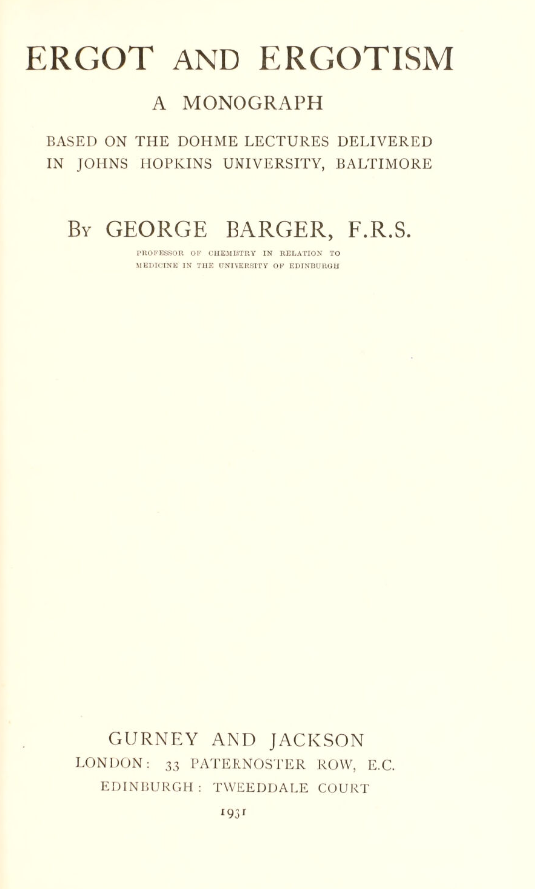
\includegraphics[height=.3\textheight]{media/1-ergotcover.png}
	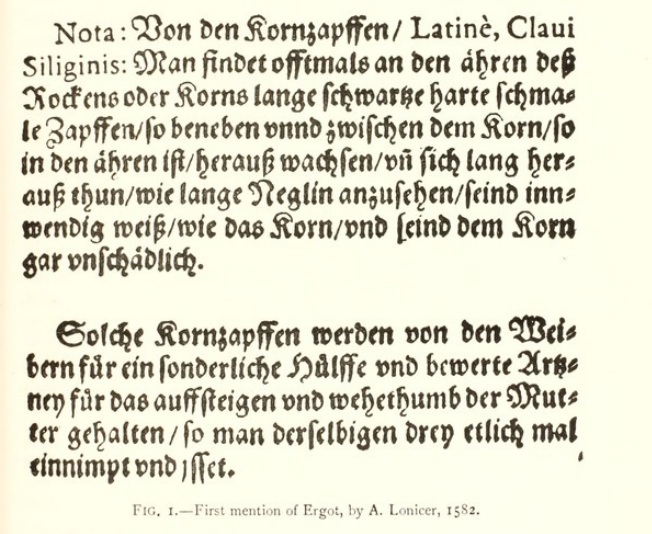
\includegraphics[height=.3\textheight]{media/1-ergotparagraph.png}
	\caption{Texto con una de las menciones más tempranas al ergot donde se descibe su uso obstétrico. La historia completa del hongo se expone con exquisito detalle en el libro \textit{Ergot and ergotism}, del que se extrae este fragmento.}
	\label{ergotbook}
\end{figure}

\subsection{Las investigaciones de Albert Hofmann.}

Recién salido de la Universidad de Zürich, el estudiante de química Albert Hofmann comenzó a trabajar en los laboratorios de la compañía Sandoz en 1929. Sandoz había investigado en las décadas pasadas los alcaloides del ergot: sustancias que, se pensaba, producían en los organismos los efectos terapéuticos y tóxicos del ergot. Si se lograba separar los componentes encargados de la contracción uterina de los responsables del ergotismo, se obtendrían medicamentos valiosísimos. Estos estudios estaban liderados por Arthur Stoll, y Albert Hofmann se propuso continuarlos bajo su supervisión.

Hofmann hizo avances rápidos aislando los componentes uterotónicos y hemostáticos, útiles como fármacos durante el parto y que hicieron del ergot un remedio tan popular en tiempos pasados; y el núcleo común de muchos alcaloides ergoticos: el ácido lisérgico (no confundir con su dietilamida, el LSD. El ácido lisérgico no es alucinógeno) (Figura \ref{alkaloids}).

\begin{figure}[H]
	\centering

	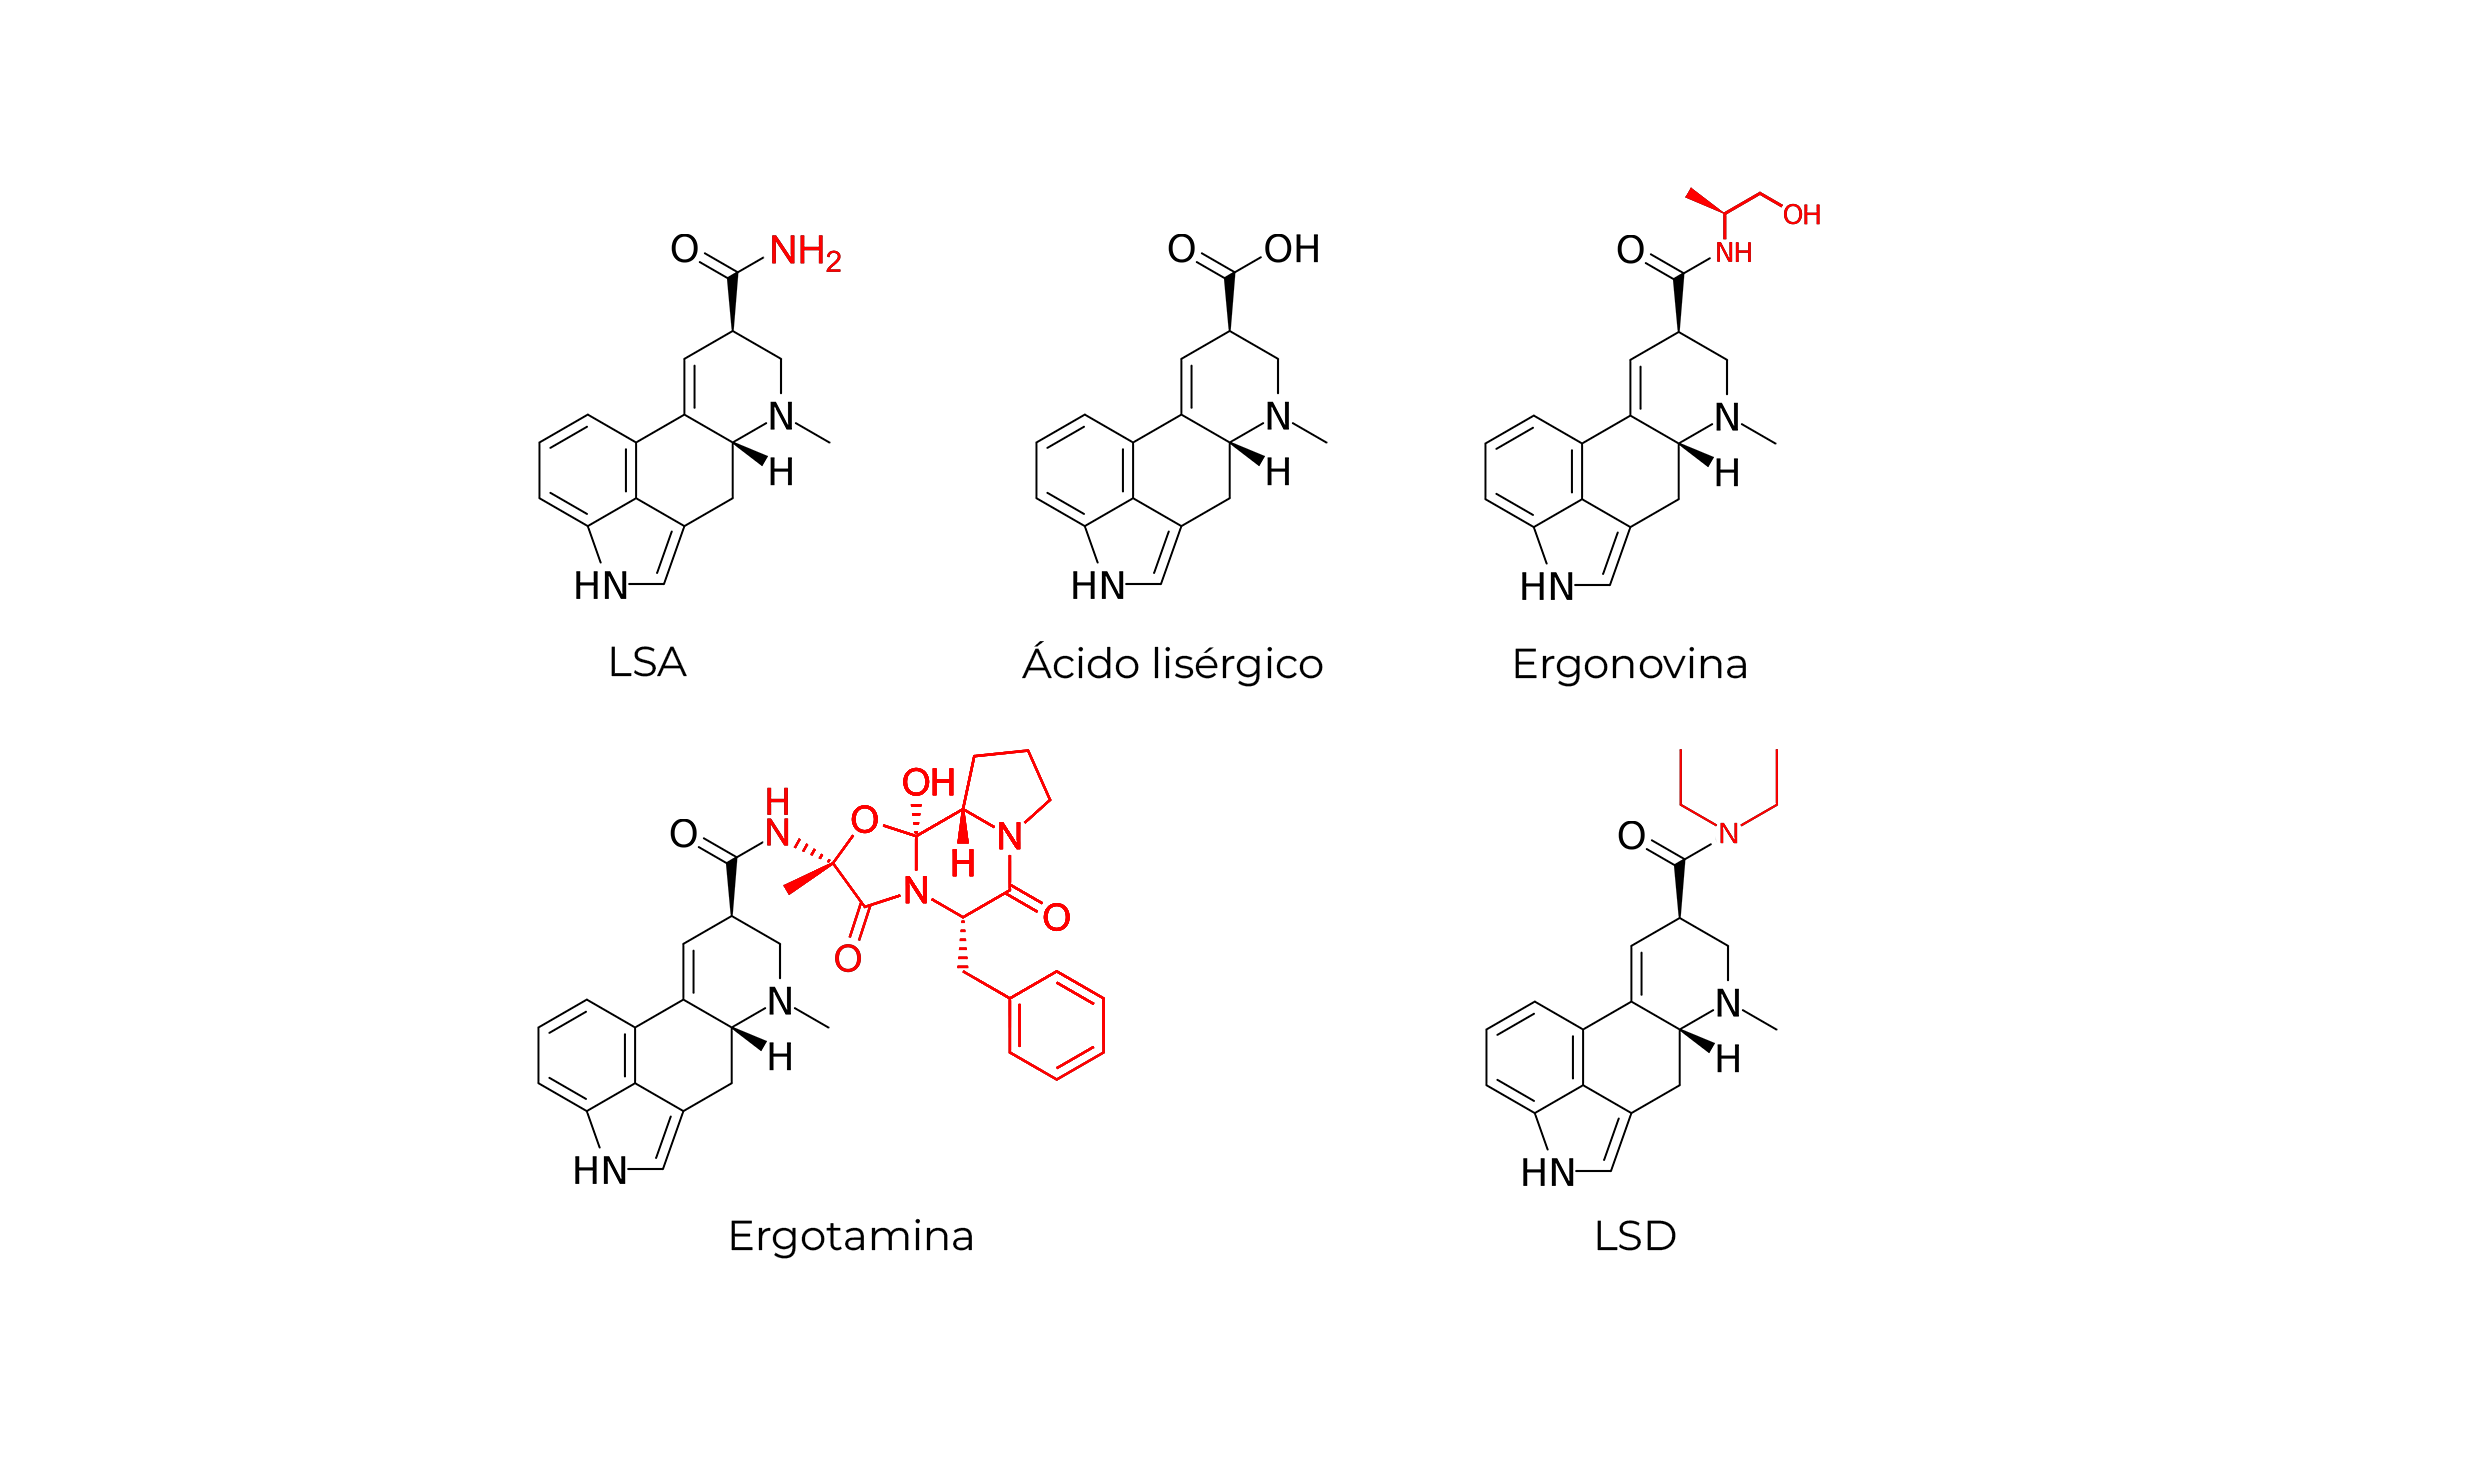
\includegraphics[width=\linewidth]{media/2-alkaloids.png}
	\caption{Muchos alcaloides del ergot son derivados del ácido lisérgico (en negro) a través de una amida con otro compuesto (en rojo). El LSD (en la parte inferior derecha) es la di-etil-amida del ácido lisérgico, es decir, el ácido lisérgico unido a dos grupos etil a través de un enlace amida.}
	\label{alkaloids}
\end{figure}

A partir del ácido lisérgico, Albert Hofmann sintetizó decenas de compuestos, el vigesimoquinto de los cuales en 1938 fue su dietilamida: el LSD-25 o simplemente LSD (Lysergsäure-Diethylamid). En primera instancia se lo consideró irrelevante y no volvió a ver la luz hasta 5 años después cuando Hofmann, intrigado por \enquote{un presentimiento de que la sustancia poseyera propiedades distintas a las inicialmente establecidas}, decidió volver a sintetizarlo. Durante el proceso se vio atacado por unas extrañas sensaciones que después comunicaría a Stoll:

% Cita
\let\oldquote\quote
\let\endoldquote\endquote
\renewenvironment{quote}[2][]
  {\if\relax\detokenize{#1}\relax
     \def\quoteauthor{#2}%
   \else
     \def\quoteauthor{#2~---~#1}%
   \fi
   \oldquote}
  {\par\nobreak\smallskip\hfill(\quoteauthor)%
   \endoldquote\addvspace{\bigskipamount}}

\begin{quote}[LSD: my problem child]{Albert Hofmann}
	\enquote{El viernes pasado, 16 de abril de 1943, me vi obligado a interrumpir mi jornada en el laboratorio en plena tarde y volver a casa, viéndome afectado por una inquietud remarcable combinada con un ligero mareo. En casa me tumbé y me hundí en una condición no desagradable de intoxicación caracterizada por una imaginación extremadamente estimulada. En un estado onírico, con los ojos cerrados (sentia que la luz del día era irritantemente deslumbradora), percibí un torrente ininterrumpido de imágenes fantásticas, figuras extraordinarias con un juego de color intenso y caleidoscópico. Después de unas dos horas, esta condición se disipó.}
\end{quote}

Teorizó que, en un descuido, un poco de LSD-25 había entrado en contacto con su piel, causando estos efectos. De ser esto cierto, la dosis activa de la sustancia tenía que ser diminuta. Para confirmarlo, decidió consumir a los tres días 0.25 miligramos, una cantidad que consideraba prudente. Sintió como si un demonio se apoderase de su mente, cuerpo y alma. Temió estar en una transición a la muerte. Había tomado en realidad dos veces y media la dósis que ahora se considera estándar. A pesar de todo su estado físico era correcto (exceptuando sus pupilas dilatadas), así que pasado el tiempo y la ansiedad, pudo disfrutar de las fantásticas imágenes que pasaban por delante de él. Para su sorpresa, no sintió ninguna clase de resaca al día siguiente, sino una sensación de bienestar que florecía en él. Veía al mundo como recién creado. El LSD produce efectos alucinógenos similares a los de la mescalina o la psilocibina (alcaloides del cactus Peyotl y las setas psilocíbeas respectivamente) en dósis decenas de veces inferiores y sin efectos tóxicos crónicos a esas dosis, siendo el principal peligro asociado - según Hofmann - lo que se hace o siente durante el estado de ebriedad. Para comprender los detalles del funcionamiento del LSD es necesario conocer en profundidad sobre qué actúa

\newpage

\section{Los fundamentos del sistema nervioso.}

El sistema nervioso es la máquina química más compleja conocida y por conocer. Todo estudio del mismo está condenado a constantes huecos teóricos y amplias fronteras, muchas en eterna penumbra. Esta condición nace de una complejidad organizativa y no una fundamental, pues los elementos individuales son en gran parte bien entendidos. Más allá de las limitaciones de la neurociencia como campo novel, el conocimiento sobre la percepción está limitado por cuestiones metafísicas. Aun después de que el lector haya aceptado su propia existencia se plantean ciertos dilemas: existen casos de pacientes que han sufrido lesiones cerebrales y muestran cambios en su comportamiento tales que se vuelven irreconocibles ante sus seres queridos. Intentar explicar tales fenómenos utilizando conceptos de alta abstracción como \enquote{personalidad} o \enquote{alma} es un interesante juego intelectual, pero también un pozo de respuestas contradictorias. Es por ello que a la hora de estudiar estos fenómenos no podemos sino limitarnos a encontrar patrones en aquéllo que podemos observar y escribir un gran \enquote{NO LO SABEMOS} en lo que lo rodea.

Lo que procede no va a ser simple, pero en esencia se resume en:

\begin{enumerate}
	\item El sistema nervioso está compuesto por células llamadas neuronas.
	\item Una neurona puede comunicarse con otra(s) por medio de señales unidireccionales.
	\item Cadenas y redes de neuronas establecen circuitos funcionales que pueden configurar desde comportamientos sencillos (como mover la pierna de forma refleja) hasta otros complejísimos (como el estado emocional).
\end{enumerate}

Alterar el comportamiento de grupos de neuronas de manera muy sutil puede provocar reacciones en cadena perceptibles a mayor escala. Esto es lo que ocurre al administrar una droga, y se verá más en detalle próximamente.

\subsection{Los bloques del sistema nervioso.}

A las puertas de la treintena de edad y buscando estabilidad financiera, Camilo Golgi comenzó a trabajar en un hospital para enfermos crónicos en Abbiategrasso. En la cocina de su alojamiento y con poco más que un microscopio y utensilios autofinanciados, montó un laboratorio al que regresaba tras cuidar de sus pacientes para continuar investigando acerca de un misterio que lo perseguía: el agente responsable de la comunicación nerviosa. Golgi desarrolló un método con el que logró teñir algunas células del sistema nervioso de un color negro. Este descubrimiento histológico tanteó la posibilidad del entendimiento de la mente, algo inimaginable en el siglo XIX. Irónicamente, su figura se vio eclipsada por la del cientifico español Santiago Ramón y Cajal que, utilizando su mismo método, construyó teorías mucho más acertadas que él.

Las células - llamadas células nerviosas o neuronas - tenían una estructura ramificada e interconectada que formaba amplias redes. Los dos cientificos diferían en un sencillo detalle: ¿eran las neuronas células independientes como decía Cajal o actuaban como un tejido continuo sin separación interna como pensaba Golgi? Este enfrentamiento se cerró definitivamente con la invención del microscopio electrónico y el descubrimiento de una breve interrupción entre neurona y neurona: el espacio sináptico (Figura 3: C1).

% Figura(s)

Este conflicto sin embargo era hijo de una guerra que se libraba desde tiempos de Descartes. La guerra entre quienes creían que el sistema nervioso actuaba como un todo y quienes pensaban que se dividía en partes funcionales localizadas. Subproductos de esta lucha fueron personas como Franz Joseph Gall que, partiendo de la localización de las partes, ideó la frenología: un método de estudio de la personalidad a través de la medición de la forma de la cabeza que posteriormente fue empleado por teóricos del racismo como justificación cientifica (Figura 4). Esta idea se veía contrapuesta a opiniones como la de Pierre Fluorens, que poniendo a prueba las tesis de Gall, concluyó que todas las partes del cerebro se encargan de todas las operaciones mentales. Una reacción no solo cientifica sino cultural, pues la reducción del alma a la actividad interna de una red de órganos era algo inaceptable para el contexto europeo.

% Figura

El pensamiento actual al respecto es algo mixto. Si bien se reconoce que tareas muy complejas como las emociones son desempeñadas en muchos circuitos distribuídos a lo largo de regiones variadas, también se acepta que estas se pueden descomponer en tareas más sencillas que generalmente sí son localizables.

\subsection{Estructura y organización.}

El entorno proporciona a los organismos un torrente continuo de información: radiación electromagnética, variaciones en la presión del aire, vibraciones en el suelo... Existen órganos con receptores capaces de reaccionar a estas variaciones en el medio: los órganos sensoriales. A las variaciones percibidas por un organismo a través de estos órganos se las denomina \enquote{estímulos} (nótese que dependiendo del nivel de abstracción un estimulo puede ser desde el tintineo de una campana hasta el impacto de un solo fotón). Cuando un órgano sensorial recibe un estimulo, este produce una señal sobre el sistema nervioso que generalmente concluye en la activación de otro órgano al que se denomina \enquote{efector}. La acción realizada se denomina \enquote{respuesta}, y si la respuesta es suficientemente compleja, la llamamos \enquote{comportamiento}.

Entre el estimulo y la respuesta actúa el sistema nervioso: un conjunto de células que conducen señales eléctricas por distintas partes del organismo. Se divide en sistema nervioso central (SNC), compuesto por el encéfalo y la médula espinal, y sistema nervioso periférico (SNP), compuesto por todos los nervios que se ramifican del anterior. El SNP actúa como una autopista de información entre el SNC y los órganos sensoriales y efectores, mientras que el SNC se encarga de integrar y procesar los aportes del SNP para ofrecer una respuesta adecuada.

Por ejemplo, ante la presencia de una tarántula en la pierna (estimulo), los receptores sensoriales en la piel enviarán señales comunicando la información al SNC por medio de cadenas de neuronas (nervios) del SNP. En este momento y tras mirar a la tarántula, el SNC, configurado a lo largo de años por experiencias pasadas con arácnidos, concepciones culturales sobre las tarántulas o por simple predisposición genética podría activar a través del SNP músculos de la pierna para zarandearla y glándulas para segregar hormonas de estrés y miedo. El SNP entonces cuenta con dos vías: la aferente (de los órganos sensoriales al SNC) y la eferente (del SNC a los órganos efectores).

No todas las respuestas necesitan al encéfalo. Muchos comportamientos reflejos están autocontenidos en circuitos de la médula espinal. Sin embargo el encéfalo ofrece una capacidad de interpretación muy útil en seres vivos más complejos.

Las células del sistema nervioso que envían y reciben señales son las neuronas, pero en el sistema nervioso también hay otras células como la glía, que sirve de apoyo para las neuronas (Figura 5). Desde la microglía con función inmunitaria hasta la macroglía, que recubre a las neuronas con una capa lipídica de mielina, las nutre controlando el paso de sustancias del torrente sanguíneo y controla las concentraciones de iones, neurotransmisores y elementos exógenos (Figura 3).

% Figura

\subsection{La neurona.}

Toda neurona está compuesta por tres partes: un soma o cuerpo celular, donde los procesos metabólicos habituales de toda célula ocurren; las dendritas, una estructura ramificada por la que entran las señales; y el axón, también ramificado y que envía señales a otras neuronas. El axón cumple una función integradora, pues en base a las diversas señales recibidas \enquote{decide} si disparar o no una señal hacia otras neuronas. Se denomina \enquote{neurona presináptica} a aquélla que envía una señal, y \enquote{neurona postsináptica} a aquélla que la recibe. Evidentemente estos son términos relativos, pues toda neurona es a la vez presináptica y postsináptica. ¿Cómo es posible la rapidísima comunicación que se observa en el sistema nervioso? Es necesario un análisis molecular.

En estado de reposo la neurona está polarizada, es decir, al igual que una pila, mantiene en todo momento una diferencia de potencial entre su interior y su exterior de unos 70 milivoltios menos. Decimos que el interior está a -70 mV respecto del exterior. ¿De dónde nace este potencial y por qué no hay un cortocircuito instantáneo que lo calme? Todo depende de un delicado equilibrio (Figura 6).

Como toda célula, la neurona está delimitada por una bicapa fosfolipídica, por ende no permite el paso de sustancias cargadas como los iones. Al no permitir el paso de iones, es imposible el flujo de electricidad, por lo que el cortocircuito mencionado no sucede. Esta bicapa sin embargo se ve interrumpida por proteínas transmembranales llamadas canales, cuya estructura forma un \enquote{túnel} por el que sí pueden circular iones. Estos canales son capaces de discriminar entre iones, dejando pasar a unos pero no a otros. Además, pueden abrirse y cerrarse bajo distintas condiciones, permitiendo o no el flujo.

Fuera de la célula, la concentración de iones de sodio (Na$^+$) es alta, mientras que dentro es baja. Por otra parte, la concentración de iones de potasio (K$^+$) fuera es baja, mientras que dentro es alta. Esta diferencia de concentración es mantenida por los riñones y la bomba de sodio-potasio, una proteína que introduce en la célula dos iones de K$^+$ por cada tres Na$^+$ que saca, consumiendo energía. Los iones entonces se ven expuestos a una fuerza electroquímica: la suma de la fuerza que intenta igualar el potencial en el exterior y el interior más la fuerza de difusión que intenta igualar las concentraciones internas y externas. Estas fuerzas producen un vaivén de iones que se desarrolla hasta alcanzar un equilibrio. El potencial interno durante este equilibrio se llama potencial de membrana.

En condiciones de reposo, los canales abiertos son más permeable a K$^+$ que a Na$^+$, por lo que, sumado a la acción de la bomba Na$^+$-K$^+$, el potencial de equilibrio es de -70 mV. Sin embargo, ciertas modificaciones fisicoquímicas pueden alterar esto. Por ejemplo, una entrada considerable de Na$^+$ puede llevar al interior de la célula a -55 mV (un potencial conocido como \enquote{umbral}). En estas condiciones, los canales iónicos de Na$^+$ que se activan por voltaje se abren, desequilibrando el sistema y causando un flujo enorme de sodio. El nuevo potencial de equilibrio en estas condiciones es de unos +55 mV, y se conoce como potencial de acción. El cierre de estos canales y la subsecuente acción de la bomba Na$^+$-K$^+$ recupera entonces el estado inicial del sistema hasta el siguiente desequilibrio.

% Figura

\subsection{Neurotransmisión.}

Los canales iónicos pueden abrirse y cerrarse debido a la unión de ciertas moléculas a las que denominamos \enquote{neurotransmisores}. A cada receptor le corresponde un solo neurotransmisor. Los neurotransmisores son liberados por la neurona presináptica, que los almacena en pequeñas vesículas. Durante el potencial de acción se abren canales de Ca$^{2+}$. La entrada de calcio causa reacciones sobre las proteínas de las vesículas y la membrana celular que producen la fusión de ambas (exocitosis). Esta fusión, que puede ser total o parcial, libera los neurotransmisores contenidos en la vesícula hacia el espacio sináptico, donde viajan hasta llegar a los receptores de la neurona postsináptica a los cuales se unen. Las moléculas que se unen a receptores son denominadas \enquote{ligandos} (Figura 3).

Al unirse a los receptores pueden hacer más o menos difícil que los canales se abran, sea directamente (en receptores ionotrópicos) o indirectamente produciendo cambios metabólicos en la célula (en receptores metabotrópicos). Si bien la acción depende del receptor y no tanto del transmisor, muchos neurotransmisores tienden a ser exclusivamente excitatorios (aumentan la probabilidad que se abran canales, aumentando también la de que se produzca una señal) o exclusivamente inhibitorios (disminuyen la probabilidad). Los aminoácidos glutamato y GABA por ejemplo son los principales encargados de la transmisión excitatoria e inhibitoria respectivamente.

Los neurotransmisores más importantes para nuestro caso son las catecolaminas (dopamina, norepinefrina y epinefrina), encargadas de funciones excitatorias, miedo, ira y recompensa; y la serotonina: crucial en la regulación del ánimo, la percepción y el sueño y muy relacionada con LSD

\subsection{Ejemplo: el reflejo rotular.}

El circuito neuronal que provoca el reflejo rotular es un ejemplo perfecto de lo expuesto hasta el momento. Estando la pierna flexionada, se percute el tendón de la rodilla. Su extensión causa un estrés sobre el cuádriceps femoral, lo cual provoca la activación de neuronas sensoriales, produciendo un impulso nervioso aferente excitatorio hasta la médula espinal. En la médula espinal se activan dos neuronas eferentes: una excitatoria hacia el cuádriceps femoral que libera acetilcolina sobre el músculo, un neurotransmisor responsable de su contracción; y una inhibitoria que evita la activación de la neurona análoga en el músculo complementario: el aductor (Figura 7). De esta manera se coordina la contracción del cuádriceps con la no-contracción (y por ende extensión) del aductor, resultando en la extensión de la pierna. Las neuronas excitatorias se comunican utilizando el glutamato como neurotransmisor, las inhibitorias: GABA o glicina. La contracción del músculo es mediada por la liberación de acetilcolina sobre este.

% Figura

Como abejas en un panal, las neuronas se agrupan en niveles de organización cada vez más complejos produciendo facultades como los sentidos y la memoria, construyendo los fenómenos emergentes que son el individuo y – quizás – la consciencia.

En estas tareas más complejas no solemos tratar con nervios ni neuronas individuales, sino que más bien observamos cómo se activan poblaciones de neuronas en regiones aproximadas del encéfalo. Estas regiones pueden interactuar unas con otras. A veces están asociadas anatómicamente, otras funcionalmente, y otras por el neurotransmisor que usan para comunicarse. Así, cuando una persona está feliz, quizás hay más actividad en tal o cual región, mientras que si está asustada, quizás las regiones que segregan este o aquél neurotransmisor se inhiben.

Lamentablemente es necesario dar cierto \enquote{salto de fe} para establecer una conexión entre psicología y neurobiología. Esto hace muy difícil tratar trastornos relacionados con la mente, pues al no comprenderse en su totalidad los fundamentos biológicos tras ellos, no es posible administrar una medicina infalible para curarlos. Este hueco de conocimiento permite la intrusión de chamanismos y vedismos, si bien en buena parte erradicados de su componente ritualístico-espiritual en la medicina moderna.

\section{El LSD sobre el cerebro.}

La introducción de entidades exógenas como el LSD u otras sustancias al organismo produce un desequilibrio con toda clase de consecuencias.

\subsection{¿Qué es una droga?}

Los organismos consumen diversas sustancias del entorno. Algunas son asimiladas inmediatamente y convertidas en materia y energía o producen excrementos. Llamamos a estas alimentos. Otras no lo son tan fácilmente: por condiciones genéticas, el cobre puede acumularse en el hígado con consecuencias graves (enfermedad de Wilson). Pero otras sustancias, en lugar de acumularse, desencadenan reacciones inmensas sobre el organismo. Estas son de especial importancia en medicina, pues al ser similares en estructura y/o función a sustancias endógenas al organismo, pueden ser utilizadas para regularlo directa o indirectamente.

Muchas sustancias pueden servir entonces como tratamiento para distintas enfermedades (como ocurre con la insulina para la diabetes). Pero por su misma naturaleza, su presencia en niveles altos en el cuerpo puede también resultar tóxica: la aspirina por ejemplo es letal en cantidades de unos 250 miligramos por kg de peso corporal (mg / kg). Por supuesto lo letal no es la aspirina en sí, sino la dosis respecto de la medida del peso corporal. Es esta doble acción de remedio y veneno la que describe la palabra griega \textit{phármakon} ($\phi\acute{\alpha}\rho\mu\alpha\kappa o\nu$). Era un hecho incluso entonces que la distinción entre remedio y veneno no depende de la sustancia, sino de la dosis.

Entre los no-alimentos encontramos sustancias que no solo actúan de manera somática (como el cianuro de potasio o el acetaminofén), sino que también inciden sobre el sistema nervioso, afectando a la percepción y la emoción (entendida como las reacciones psicofisiológicas internas del individuo ante estímulos importantes). A estas sustancias las llamamos \textit{drogas}.

Es importante notar que el término \enquote{droga} es polisémico, y a veces se usa para denominar exclusivamente a sustancias con efecto sobre el SN, mientras que otras se emplea para referirse a cualquier cuerpo químico utilizado en medicina (la palabra \enquote{\textit{drug}} recibe este uso particularmente en la lengua inglesa).

Por último es importante reconocer que muchas drogas son ilegales y, como tal, el término guarda otro significado en el ámbito del derecho. Históricamente la relación de la humanidad con las drogas ha sido asunto de controversia (véase el ejemplo del vino en la Antigua Roma), y de manera cultural o sistemática se ha perseguido el uso de unas u otras. En torno al último tercio del siglo XX se establece una normativa más estricta en países como Estados Unidos con el Controlled Substances Act y \enquote{droga} pasa a designar a cualquier sustancia así designada por este estatuto.

Para evitar ambigüedades, en este documento emplearemos las siguientes definiciones:

\begin{itemize}
	\item Fármaco: cualquier sustancia utilizada como tratamiento para una enfermedad.
	\item Droga: cualquier sustancia que interactúa con el sistema nervioso produciendo cambios en la percepción y la emoción.
\end{itemize}

\subsection{Terminología}

Existe un conjunto de términos asociados tanto a drogas como a fármacos que definimos cuantitativa y cualitativamente. En primer lugar tenemos aquéllos referentes a la dosis. Distintos organismos difieren en sus características particulares y no reaccionarán de la misma manera a dosis iguales, es así que nuestras afirmaciones serán estadísticas y no concretas.

Es común administrar una dosis determinada a una población y observar sus efectos. La \textit{dosis efectiva media} (ED50) es aquélla que produce los efectos deseados sobre el 50\% de los individuos a los que se da (puede haber distintas dosis efectivas dependiendo de los efectos que se desee producir). La \textit{dosis letal media} (LD50) es aquélla suficiente para acabar con la vida del mismo porcentaje de población. De estas dos se extrae el margen de seguridad, que es la proporción entre dósis activa media y dósis letal media.

Tanto fármacos como drogas pierden parcial o totalmente su efecto con el uso continuado, este fenómeno es conocido como \textit{tolerancia}. Repetidas dosis diarias de aspirina generan una tolerancia que la hace mucho menos efectiva. Esta capacidad de adaptación del cuerpo no es igual para todas las sustancias, por lo que la tolerancia que induce cada una ha de ser estudiada individualmente.

En la literatura relacionada a las drogas se suele usar a la tolerancia como medida sinónima de propensión al abuso. Si bien razonable, se puede matizar. Ciertamente una droga como la heroína generará una rápida adaptación, por lo que el usuario, para sentir los mismos efectos, habrá de dejar un margen entre uso y uso o, como es común, aumentar la dosis. La adaptación del organismo al fármaco sin embargo no es pareja, y un individuo puede dejar de percibir los efectos relajantes de un opioide pero seguir sufriendo la misma depresión respiratoria. Un aumento de la dosis en este caso plantea el riesgo de intoxicación aguda. Incluso si se consigue una adaptación pareja, el uso continuado de la droga termina generando una intoxicación crónica, como es habitual en casos de alcoholismo. Un menor grado de adaptación implica límites de toxicidad más rígidos, reduciendo el riesgo de intoxicación crónica pero haciendo más fácil alcanzar dosis perjudiciales o letales.

Que el cuerpo se adapte a fármacos supone cambios metabólicos internos que hacen que el organismo necesite la presencia de la sustancia para mantener su equilibrio. Se dice entonces que el cuerpo ha generado \textit{dependencia} a la sustancia. Cuando la sustancia es eliminada --- por ejemplo por interrumpirse su uso continuado --- se produce un fenómeno de desestabilización que se manifiesta en reacciones mensurables conocido como \textit{síndrome de abstinencia}. Uno empieza a vislumbrar aquí los mecanismos biológicos que conducen a la adicción, esto es, la búsqueda compulsiva de nuevas dosis, sin embargo hemos de hacer un comentario adicional al respecto.

\newpage

\subsection{Adicción y dependencia.}

Mismos estímulos provocan distintas respuestas dependiendo de variables internas como el hambre o el estado anímico. Ante la presencia de agua y alimento, el depredador prioriza aquélla necesidad más urgente en ese momento. A ese conjunto de variables internas y su influencia sobre las externas lo llamamos \textit{motivación}. La mayoría de las motivaciones buscan saciar un desequilibrio interno a corto plazo como la sed, pero algunas expanden su vista a imperativos biológicos como la perpetuación de la especie.

Cuando un agente estimula los sistemas de recompensa del cerebro de manera artificial – llegando a predominar sobre recompensas naturales, incluso en detrimento físico o psicológico del individuo – se dice que existe una \textit{adicción}. La adicción se define como un síndrome crónico caracterizado por la búsqueda compulsiva de cierta droga, incluso ante consecuencias negativas físicas y personales.

Este fenómeno es estudiado principalmente en animales. Por ejemplo, cuando una rata es encerrada y provista de una palanca con la que estimular eléctricamente ciertas regiones de su cerebro, la rata tirará de la palanca incluso en condiciones de inanición, llegando a ignorar la comida que se le ofrezca. La persecución de una mete artificial en perjuicio de la necesidad biológica forma un paralelo interesantísimo con la adicción a drogas. Comprender las vicisitudes de la adicción implica entender los sistemas de recompensa del cerebro, algo que aún se está investigando.

Al analizar la actividad cerebral que suscitan distintos comportamientos hedónicos observamos que ciertas regiones muy concretas se activan de manera consistente. Una de estas regiones es el \textit{área tegmental ventral} (VTA por sus siglas en inglés), una región del cerebro con muchas proyecciones al \textit{núcleo accumbens} (NAc). La comunicación entre estas dos zonas se realiza por medio de un neurotransmisor llamado \textit{dopamina}, y las neuronas que la utilizan son \textit{dopaminérgicas} (Figura \ref{ratbrain}).

Algunas drogas como la cocaína o las anfetaminas son capaces de fortalecer la transmisión dopaminérgica, incrementando la actividad de los sistemas de recompensa como el de la VTA. Estas drogas no solo producen adicción física por su síndrome de abstinencia, sino que, debido a esta perturbación neuronal, causan también adicción psicológica.

\begin{figure}[H]
	\centering
	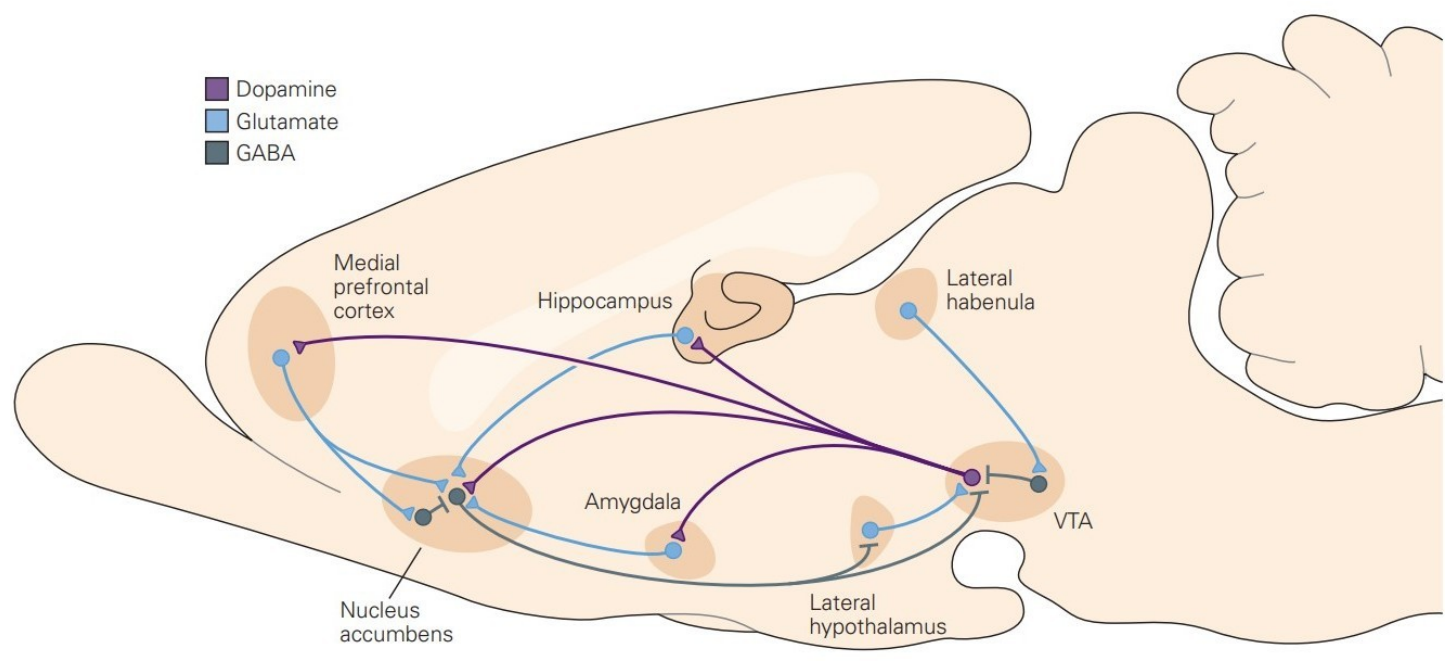
\includegraphics[width=\linewidth]{media/8-ratbrain.png}
	\caption{Esquema de proyecciones de la VTA en el cerebro de un ratón. Al activarse la VTA, neuronas dopaminérgicas (en morado) forman proyecciones excitatorias hacia distintas partes del cerebro (hipocampo, amígdala, NAc...) produciendo la emoción de recompensa.}
	\label{ratbrain}
\end{figure}

Esta explicación de la adicción sin embargo sigue sin ser completamente sólida. Identificar la dopamina con un \enquote{neurotransmisor del placer} es incorrecto. En ocasiones la dopamina señaliza respuestas negativas, y estudios más recientes asocian su liberación a un \enquote{error en la predicción}.

Además, la activación de neuronas dopaminérgicas es solo uno de los componentes de todos los procesos neuronales que ocurren durante la emoción de recompensa. Ratas carentes de dopamina aún exhiben comportamientos hedónicos ante el azúcar y la cocaína, lo que indica que este neurotransmisor no es el único factor relevante.

Peor aún, el patrón de comportamiento de realizar algo repetidamente incluso en detrimento propio puede aplicarse a conductas como el juego, la comida o el sexo, áreas complicadísimas de estudiar, pues es imposible construir un modelo humano a partir de una rata con adicción a ir de compras. Hasta en roedores es difícil hallar patrones deterministas: grupos de ratones no desarrollan adicción a la cocaína en las mismas proporciones estando totalmente aislados que dentro de \enquote{ambientes enriquecidos} dotados de compañeros, tubos de polietileno y pelotas.

¿Qué paralelismos se pueden trazar entre el comportamiento de una rata y el de un humano? ¿Cómo se manifiesta la adicción a escala neuronal y cómo se relaciona realmente a las drogas? Nos topamos con el mantra repetido durante toda investigación neurocientifica: no lo sabemos. Desprovistos de afirmaciones universales, nos vemos obligados a analizar los efectos concretos del LSD.

\newpage

\subsection{Farmacología del LSD.}

La dietilamida del ácido lisérgico es una droga semisintética derivada del ácido lisérgico extraído del ergot. Posee cuatro estereoisómeros, es decir, cuatro sustancias hermanas estructuralmente: l- y d- LSD y l- y d- iso-LSD. Solo el d-LSD es psicoactivo, y es al que nos referimos al decir \enquote{LSD}. Es hidrosoluble y se derrite a 83°C, y debido a su fragilidad ante la luz, la temperatura y la humedad suele ser conservado en su forma de sal de tartrato. Debido a su alta biodisponibilidad, la vía de administración más común es la oral. Originalmente se realizaba a través de ampollas, pero se popularizó el consumo a través de papeles secantes o terrones de azucar bañados y colocados sobre la lengua. Distintas dosis de LSD configuran distintos efectos.

En un individuo de entre 50 y 70 kg de peso, la mínima dosis reconocible es de 25 $\mu$g y produce algunas alteraciones cognitivas. La dosis estándar está entre 70 y 100 $\mu$g, y produce una acción de 6 a 10 horas, ya con efectos visionarios. A partir de 300 $\mu$g comienzan las dosis altas, con efectos intensos durante más de 10 horas.

La dosis letal media en distintos animales está entre 0.3 y 16.5 mg / kg, siendo 1 mg / kg en monos. No se ha encontrado la dosis letal en humanos, pues no se conocen casos de muertes por LSD. En una ocasión ocho individuos confundieron LSD con cocaina y consumieron una dosis altísima, hallando 1-7 mg de la sustancia por cada 100 mL de su sangre. Sufrieron de estados comatosos, hipertermia, vómitos, sangrados gástricos y problemas respiratorios, pero con tratamiento hospitalario, todos sobrevivieron sin secuelas. Es preciso afirmar entonces que el margen de seguridad del LSD es extraordinariamente alto.

El LSD presenta una tolerancia elevadísima. Después de dosis de entre 5 y 100 microgramos administradas durante 3 a 6 días, los voluntarios desarrollan una fuerte tolerancia. Esta desaparece en torno a los 4 días sin uso. Más allá de la tolerancia, existe un consenso general en que el LSD no es adictivo, es decir, no produce los comportamientos de búsqueda compulsiva de más dosis.

Se observa que esta sustancia tiene unas propiedades excepcionales, sin embargo que sea farmacológicamente segura no implica que su uso en general sea seguro. Existen casos documentados de autolesión y suicidio bajo los efectos de esta droga, si bien el número es reducido. Más detalles al respecto se dan en el capítulo sobre su historia contemporánea.

\newpage

\subsection{Efectos del LSD.}

Una dosis estándar de LSD altera de manera significativa el estado de consciencia, con una tendencia a la euforia, es decir, un intenso estado de felicidad y bienestar; un impulso en la capacidad de introspección y la estimulación de procesos Freudianos primarios, es decir, los deseos instintivos se desatan, inhibiendo la influencia del ego y la sociedad sobre el individuo. El efecto más característico son las alteraciones en la percepción como ilusiones, visiones, pseudoalucinaciones, sinestesias --- la capacidad de cruzar sentidos --- y alteraciones en el pensamiento y la percepción temporal. Mención especial merecen los cambios que provoca sobre la percepción de uno mismo y la función del ego. El LSD (especialmente en dosis altas) debilita la frontera que separa al \textit{yo} del resto del mundo, un fenómeno conocido como \enquote{disolución} o \enquote{muerte del ego}.

La potencia inigualada del LSD es un arma de doble filo, pues al igual que es capaz de proporcionar una buena experiencia y efectos psicológicos positivos a largo plazo, también puede provocar experiencias traumáticas (llamadas coloquialmente \enquote{malos viajes}) con efectos negativos como cambios de humor y, a veces, escenas retrospectivas que pueden resultar nocivas. Es difícil estudiar los efectos del LSD en el pensamiento, pues no podemos introducirnos en la mente de nadie y la dosis estándar ya es suficiente para dificultar la comunicación durante los experimentos. Se puede decir que el efecto del LSD reduce la destreza en pruebas de atención y concentración, habilidades psicomotoras y aritméricas, memoria visual y noción temporal – se tiende a sobreestimar los intervalos temporales. Los procesos de aprendizaje no se ven afectados. Ciertas interpretaciones argumentan que las funciones intelectuales sufren un regreso a un estado más temprano de desarrollo. No se conoce ninguna facultad perjudicada de manera crónica por el uso de LSD. En muchas personas produce mareos y agitación interna.

\subsection{Mecanismo de acción: el sistema serotoninérgico.}

La serotonina (también denominada 5-hidroxitriptamina o 5-HT) es un neurotransmisor que se produce a partir del triptófano en pocas neuronas (contadas en millares). Estas neuronas se ubican principalmente en los \textit{núcleos del rafe} del mesencéfalo, y proyectan sus conexiones a regiones como el hipocampo, la corteza cerebral, el NAc y núcleos dopaminérgicos como la VTA, entre otras (Figura \ref{pathways}). Es particularmente importante la conexión de los núcleos del rafe con el \textit{locus coeruleus} (LC), pues esta región se encarga de la liberación de noradrenalina y tiene conexiones con el cerebelo, el tálamo, el hipotálamo, la corteza y el hipocampo.

Es evidente que, a pesar de ser reducidas en número, las abundantes conexiones salientes de las neuronas serotoninérgicas (hasta 500.000 por neurona) hacen de la 5-HT un neurotransmisor crucial en procesos tan diferentes como la regulación del ánimo, la temperatura corporal y hasta el tracto gastrointestinal. La deficiencia en niveles de serotonina se asocia a trastornos depresivos, que son tratados con varias formas de psicoterapia y fármacos antidepresivos (normalmente inhibidores selectivos de recaptación de serotonina o SSRIs, como la fluoxetina y la sertralina).

El sistema serotoninérgico está también relacionado con el filtro de información en el cerebro. No todos los estímulos del medio son igual de importantes, y algunos --- como el sonido del oleaje --- son continuos y repetitivos, por lo que no merecen atención constante. El cerebro tiene una capacidad de procesamiento limitada, por lo que automáticamente descarta esta información para dejar espacio a otra más valiosa, evitando además una sobrecarga sensorial. Una alteración en este sistema de cribado podría explicar los efectos estimulantes y alucinógenos del LSD.

La estructura molecular del LSD es similar a la de la serotonina, lo que le permite unirse a algunos de sus receptores, aunque con menos fuerza que la propia serotonina (se dice que es un \textit{agonista parcial}). Esta interacción altera el comportamiento del sistema serotoninérgico, aunque no se conoce plenamente cómo. Las neuronas del sistema serotoninérgico cuentan con 14 receptores de serotonina distintos (y se teoriza un 15$^\circ$), siendo algunos inhibitorios y otros excitatorios, y la gran mayoría metabotrópicos (es decir, que no controlan directamente la apertura de un canal, sino que modulan la actividad de la neurona por medio de segundos mensajeros). Estos receptores se nombran como \enquote{5-HT$_{\textrm{XY}}$} (receptor de serotonina Y de la clase X).

Concretamente actúa como agonista parcial en los receptoers 5-HT$_{\textrm{1A}}$, 5-HT$_{\textrm{2A}}$ y 5-HT$_{\textrm{2C}}$, pero también sobre receptores de otros neurotransmisores como el dopaminérgico D$_2$ y el adrenérgico $\alpha_2$. Un efecto secundario de estimular los receptores 5-HT$_{\textrm{2A}}$ es la activación de transmisión glutamatérgica en la corteza frontal. Este es un patrón clave compartido por el LSD y otros alucinógenos serotoninérgicos, y se cree que esta activación podría causar una perturbación en los sistemas de filtro de procesos sensoriales y cognitivos. La tolerancia podría ocurrir debido a una reducción en la densidad de receptores 5-HT$_{\textrm{2A}}$.

\begin{figure}[H]
	\centering
	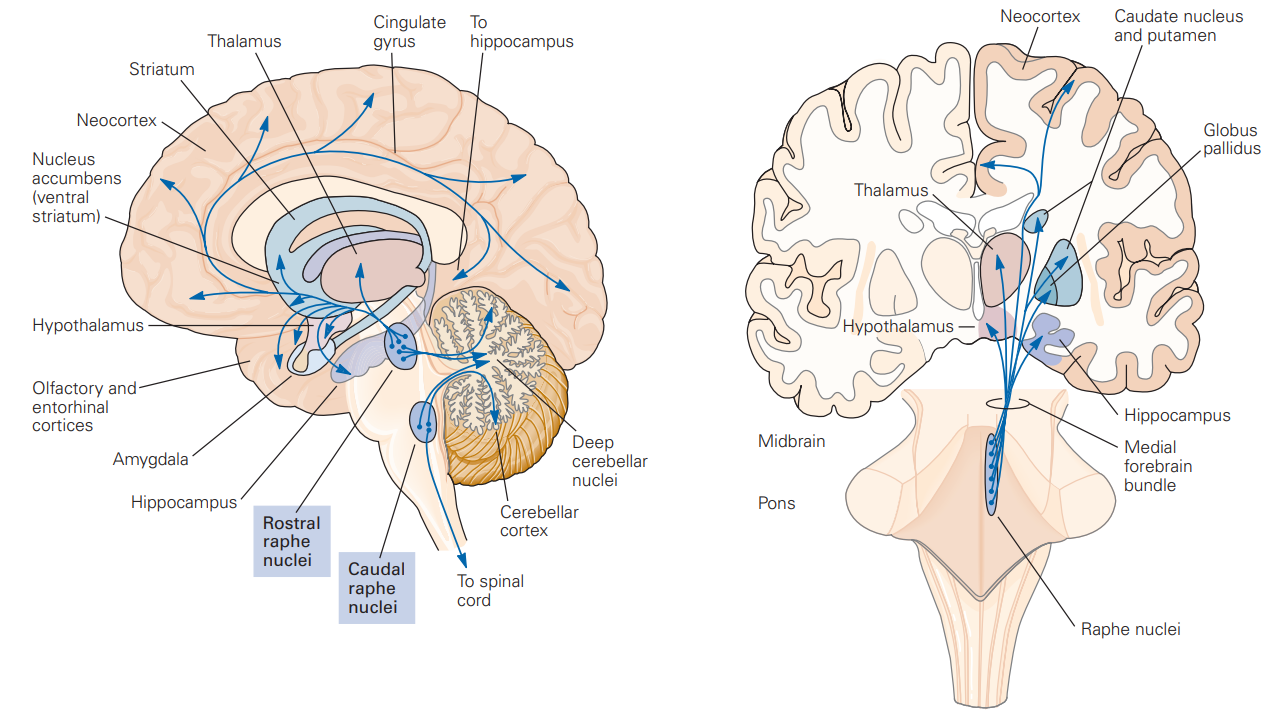
\includegraphics[width=\linewidth]{media/9-pathways.png}
	\caption{Rutas serotoninérgicas encefálicas. Las neuronas serotoninérgicas nacientes de los núcleos del rafe se proyectan hacia numerosas regiones encefálicas.}
	\label{pathways}
\end{figure}

\newpage

\section{Historia contemporánea y usos.}

Menos de una hora después de que Hofmann se administrase la dosis, estaba claro que el LSD era el culpable de su anómalo estado. Ayudado por su asistente, regresó en bicicleta a casa atravesando un paisaje ondulante. Tumbado en el sofá, su alrededor se tornaba grotesco. Su vecina que traía leche se convirtió en una malvada bruja. Estaba aterrorizado de que su experimento dejase a una familia sin padre, mas cuando llegó el médico, este no aconsejó más que dejar pasar el tiempo, pues sus constantes vitales eran correctas. Gran acierto, ya que de aquél escenario macabro descendió a la realidad, pudiendo disfrutar del residuo de sinestesias e imágenes caleidoscópicas. Al día siguiente se encontraba con la cabeza totalmente fresca, pudiendo recordar toda su experiencia.

Hofmann visionó en el LSD una droga de enormísima utilidad en farmacología, neurología y particularmente en psiquiatría. Jamás habría podido anticipar sin embargo que fuese a ser utilizada de manera recreativa después de lo vivido.

Tras informar a su supervisor, el departamento farmacológico de Sandoz se puso manos a la obra a estudiar la tolerancia y toxicidad de la sustancia. Los primeros exámenes en animales mostraban a gatos que observaban a la nada y en lugar de atacar a ratones, los miraban horrorizados. Las arañas construían telas más eficientes en dosis bajas pero rudimentarias en dosis altas. Al introducirse en una comunidad de chimpancés, incluso si solo unos pocos individuos lo tomaban, el grupo entero entraba en conflicto debido a que estos no seguían las leyes jerárquicas de su tribu.

Demostrada la seguridad del LSD y probado sistemáticamente en humanos, Sandoz lo comercializó como un fármaco experimental: el Delysid. Entre sus usos se citaba además la autoexperimentación del psiquiatra para ganar perspectiva sobre la emoción interna de sus pacientes, pues la experiencia servía como modelo de distintas afecciones.

\subsection{Terapia psicodélica, arte y recreación, prohibición.}

El LSD no actúa como un medicamento \textit{per se}, es decir, no arregla - que sepamos - ningún desequilibrio químico como sí lo hace un antidepresivo. Sin embargo, dados los peculiares efectos que produce sobre la consciencia, sus usos como fármaco auxiliar en psicoterapia y psicoanálisis han sido muy abundantes. Al llevar al extremo el estado interno del usuario y hacer que reaparezcan recuerdos olvidados (en forma de \enquote{reviviscencia}), el LSD es una herramienta útil para liberar material reprimido, haciéndolo eficiente para tratar el trauma. Además, al disolver la barrera entre el tú y el yo, facilita el desprendimiento de problemas centrados en el ego. También se ha utilizado en pacientes terminales de cáncer que desarrollan mucha tolerancia a los analgésicos, aunque esto plantea cuestiones éticas. La experiencia de disociación corporal impide que el dolor penetre en la consciencia y facilita el coraje para afrontar la propia muerte. Este uso requiere supervisión y una preparación especial, a menudo siendo útil que un psicoterapeuta o una figura religiosa guíe la experiencia. El célebre escritor Aldous Huxley pidió en su lecho de muerte a su mujer ser inyectado con 100 microgramos, varias dosis si fuese necesario.

A principios de los 60 el LSD se extiende como la pólvora por occidente, con una influencia particular sobre la sociedad estadounidense que se ve acompañada casual o causalmente por el nacimiento del movimiento hippie. El doctor Timothy Leary de la universidad de Harvard fue una figura muy relevante en la difusión de LSD en los Estados Unidos. Realizó exámenes sobre su uso en miembros del clero, convictos y artistas, aunque sus obras rápidamente perdieron el carácter cientifico y fue expulsado de la universidad. Convertido al hinduísmo, pasó a ser uno de los principales líderes del movimiento hippie. Con el grito estampado hasta la saciedad de \enquote{Turn on, tune in, drop out}, alentaba a la juventud a consumir LSD (turn on) para explorar su mundo interior (tune in) y finalmente desprenderse de la vida burguesa, los estudios, el trabajo y toda cadena con el cántico \enquote{drop out} (Figura 10).

% Figura

Esta subversión de las estructuras convencionales era un pronunciamiento abierto que desafiaba - recordando a los chimpancés que perdieron su estructura jerárquica - a toda autoridad social y política. El Dr. Leary fue arrestado en Kabul y encarcelado por posesión de drogas. En 1976, ya libre, se mantuvo ocupado con cuestiones como la relación entre el SNC y el espacio interestelar.

El LSD siguió una ruta histórica similar a la de la mescalina: comenzó como un químico de interés en agrupaciones cientificas y psiquiátricas y se inmiscuyó entre intelectuales. Las experiencias estéticas e introspectivas inducidas lideraban el proceso creativo de los artistas, y de sus numerosas obras nació el arte psicodélico, que comprende toda creación realizada tras el uso de LSD y otros psicotrópicos como la mescalina o la psilocibina. El libro \textit{Psychedelic art} contiene una recopilación excelente de este género.

En la música grupos tan populares como los Beatles fueron marcados por esta sustancia. Discos como \textit{Revolver}, o \textit{Sgt. Pepper’s Lonely Hearts Club Band} y canciones como \textit{Lucy in the Sky with Diamonds} (título que hoy sirve de alias a esta droga) recibieron una influencia estética propia del LSD. En conjunto, bandas coetáneas como Pink Floyd, Jefferson Airplane y The Grateful Dead concibieron el género del \textit{rock psicodélico}.

El LSD se introdujo también en las clases populares. Hofmann había previsto curiosidad por parte de los artistas e intelectuales, pero jamás pensó que su creación fuese a ser empleada como un embriagador común, y este uso provocó varios incidentes. Los experimentos clínicos y universitarios con la droga pasaron de ser compartidos en publicaciones cientificas a ser presentados delante de todo el mundo en revistas y periódicos, donde las conclusiones eran exageradas. Los reportajes acerca de esta droga ya no se daban en tercera persona, sino que los mismos periodistas la consumían y relataban posteriormente sus experiencias. En los mercados estadounidenses aparecían libros relatando los efectos del LSD, muchas veces exaltándolos.

Toda esta literatura implantó en la cultura popular una idea falsa: que el solo uso de esta medicina era suficiente para lograr efectos milagrosos. Bajo semejante concepción, comenzó el imperio de la autoexperimentación. Los sesenta, con una crisis existencial de la sociedad estadounidense, la completa legalidad de la sustancia y la expiración de las patentes de Sandoz hicieron al LSD omnipresente. Como era de esperar, las experiencias populares se parecían más a las primeras de Albert Hofmann. \enquote{Malos viajes}, desorientación y pánico eran el producto habitual del experimento propio, a veces provocando accidentes y crímenes.

Entre 1964 y 1966 la polémica del LSD reinaba, con entusiastas diciendo que era una sustancia mágica y otros que señalaban los accidentes y crímenes que se cometian bajo sus efectos. Sandoz sufrió demandas masivas acerca de las propiedades de la sustancia. Finalmente en agosto de 1965 dejaron de producir y exportar públicamente el Delysid. A cambio, ofrecieron entregarlo a investigadores cualificados de todo el mundo, con asistencia tanto técnica como en muchos casos financiera. Sumado a una detallada descripción en el \enquote{Catalogue of Literature on Delysid}, con la que se inhibió en buena medida el uso indebido.

Sandoz sin embargo no podía controlar todas las posibles excepciones. Las ideas erróneas en circulación y la total ausencia de legislación forzaron a Sandoz a cesar la producción de LSD y de alucinógenos similares como la psilocibina. A continuación siguió el Convenio sobre Sustancias Psicotrópicas de la ONU y el establecimiento de estatutos como el Controlled Substances Act en Estados Unidos, que no solo prohibía su posesión y distribución, sino que descartaba cualquier uso terapéutico de la sustancia. Su asociación a una \enquote{droga de la locura} disuadió a los psiquiatras de continuar empleándolo. El LSD, como condenado por una trágica maldición familiar, fue llevado al ostracismo al igual que su padre el ergot tres siglos antes.

El declive en uso de LSD ha afectado notablemente a su producción. En estudios psiquiátricos y neurobiológicos se ha visto sustituído por sustancias como la psilocibina encontrada en las setas alucinógenas, no solo por su semejanza en farmacología y efectos, sino porque su tiempo de acción más breve facilita su estudio. Como droga ilegal también se ha visto desplazado por derivados del cáñamo como el hachís y drogas sintéticas como la heroína y las anfetaminas, siendo habitualmente más tóxicos los sustitutos.

\subsection{Riesgos asociados al LSD.}

Actualmente la legislación no atribuye usos terapéuticos al LSD. Existen opiniones contrarias que argumentan que no hay peligro en el uso en entornos profesionales, algunas llegando a afirmar que el existente fuera de estos está relacionado con la clandestinidad y no con la sustancia. Es innegable que el uso de LSD está asociado a un conjunto de riesgos que deben ser conocidos tanto si se hace en un entorno profesional con supervisión médica como si no.

La desorientación intrínseca a todo experimento con LSD hace imposible descartar episodios de crisis, por más que se pueda minimizar mediante preparación. En los peores casos, la psicosis inhibirá la percepción de riesgo del individuo, produciendo accidentes fatales. En su defecto, una experiencia con visiones mortiferas puede conducir al suicidio. Aun si no son casos tan comunes, han de servir de advertencia. Frank Olson, un doctor estadounidense, consumió altas dosis de LSD sin su conocimiento. Se suicidó saltando por una ventana. Había sido víctima de experimentos farmacológicos del ejército estadounidense, y no fue hasta pasados 15 años que, con la revelación del proyecto MK Ultra, el director de la CIA William Colby y el presidente del gobierno Gerald Ford presentaron sus disculpas a la familia.

Es importante también analizar si el LSD es el fármaco óptimo para el bienestar del paciente, suministrándolo solo en los casos adecuados. Como el LSD intensifica el estado mental del momento, ofrecérselo a un paciente con la intención de curar un mal ánimo puede ser muy perjudicial. Tampoco debe ser utilizado sobre personalidades inestables, como aquéllas con tendencia a la psicosis. Esto incluye por lo general a la gente joven.

Es necesario un comentario acerca del uso personal que recibe el LSD. Existe un problema intrínseco al uso personal de cualquier droga. Si por definición estas actúan sobre el sistema nervioso afectando a la emoción y la percepción - y nuestro juicio se basa precisamente en estas facultades - entonces nuestra toma de decisiones se verá comprometida, incluyendo la propia decisión de consumir la droga. Ideas aceptadas o rechazadas en un estado de conciencia pueden no serlo en otro incluso a pesar de realizarse una planificación previa. Esta cuestión plantea un debate acerca de la relación del libre albedrío con el sistema nervioso, pero no lo trataremos.

Es imposible realizar un estudio cientifico acerca del uso personal de LSD, ya que de establecer un entorno controlado y realizar un seguimiento de cada individuo, el uso dejaría de ser personal. Dependemos entonces de la \enquote{sabiduría popular} relatada por periodistas y particulares como el propio Albert Hofmann. En diversas fuentes se habla por ejemplo del concepto de \enquote{set y setting} como determinante para que los sentimientos durante una experiencia sean predominantemente positivos. Se denomina \enquote{set} al conjunto de factores internos como el estado de ánimo previo y las expectativas, y \enquote{setting} a los factores externos como el carácter del entorno, su iluminación, su ruido ambiente o las personas presentes. También se menciona la importancia de una persona de confianza como sustento emocional capaz de solicitar asistencia médica en caso de ser necesario. Se hace especial énfasis en la dosis, recomendándose empezar por unas muy bajas y llevar un registro con los efectos de cada una.

Finalmente es menester recordar que el LSD es ilegal, y que en consecuencia el mercado negro es la única vía de obtención. Esto plantea riesgos totalmente ajenos a los farmacológicos. Al no estar regulados, la pureza de los productos clandestinos es desconocida, y es común encontrarlos contaminados por otras sustancias. Además del problema de la pureza está el de la dosis: incluso si se adjunta la medida en microgramos (también llamados \enquote{\textit{gammas}}), esta puede estar alterada. Dada la abismal diferencia entre dosis de 25, 100 y 600 microgramos de LSD, la incertidumbre al momento de consumir un producto clandestino hace mucho más comunes las malas experiencias.

\section{Conclusion.}

Even after this study I find myself filled with contradictions and I'm incapable of offering a consistent opinion on the moral matters. Is psychedelic therapy a potential replacement to conventional therapy or just a complement? Being able to use a substance without restrictions is freedom or slavery for users? Albert Hofmann himself ended up calling his creation a \enquote{problem child}. As with any big discovery --- the printing press, the steam engine, the Internet --- society needs some time to adapt.

Having read its historical background, removing the prohibition of its therapeutic use could make up for a very interesting field of research. Understanding serotonin's role in psychic and metabolic proceses and constructing an evolutionary map on its procedence could assist on the comprehension of brain circuits as functional components of conscious experience.

It's safe to state that any attempt to reintegrate LSD as a pharmaceutical in society won't happen without authorization from the law. Because it's such an unstable compound, harmed both by air and light, lab material and very broad knowledge on chemistry are mandatory for its synthesis and manipulation. Not the same can be said about other hallucinogens. Because they come from vegetal and fungal sources, mescaline, DMT or psylocibin are much more accessible. It's then practically impossible to completely prohibit hallucinogens (and in truth, any drug) due to the decentralized nature of their manufacture.

After this study it's possible to establish a series of statements whose truth I consider non-negotiable:

\begin{itemize}
	\item The complete elimination of a substance that comes from a fungus or plant that is easy enough to grow is impossible (or at least very expensive).
	\item Some drugs are used or have been used with therapeutic ends.
	\item Some drugs are used or have been used with recreational ends.
	\item A drug's usage implies personal and social risks.
	\item If this usage is done without the necessary knowledge, the risk can be fatal.
\end{itemize}

Which conclusions should be drawn from this is a deep topic for debate which involves psychiatrists and psychologists, but also historians, philosophers and governments. Two main discussions exist here. First, the one that questions whether the use of a certain drug is problematic. For example, many civilizations through history have used opium and laudanum as sources of analgesia and entertainment, and now they are illegal. The second question comes into place: the one referring to prohibition. In some places like the Netherlands it's considered that the use of these substances is something negative, but even then they have eliminated prohibition. The official reason is that this \enquote{prevents people who use soft drugs from coming into contact with hard drugs}, a certainly pragmatic way to handle the situation.

The disagreement is far from closed, however, knowing that some drugs will be perpetually in our society --- and that surrounding them with mysticism will only increase the number of accidents --- the need for information on their use and risks is needed.


% Bibliografía

\nocite{*}
\bibliographystyle{IEEEtran}
\bibliography{refs}

\end{document}
